%%%--- Template for master thesis at SfS
%%%--- Modified template with more comments and examples -- SG, 11/06/09
%%%------
\documentclass[11pt,a4paper,twoside,openright]{report}
%%not needed \usepackage{E}
\usepackage[english]{ETHDAsfs}%--> ETHDASA + fancyheadings + ... "umlaute" 
%  + sfs-hyper -> hyperref 

\usepackage{amsbsy}%% for \boldsymbol and \pmb{.}
\usepackage{amssymb}%% calls  amsfonts...
%or \usepackage{german8}%-- =  german  +  isolatin1
\usepackage{graphicx}%-- f�r PostScript-Grafiken (besser als  psfig!)
%\usepackage[draft]{graphicx} % grafics shown as boxes --> faster compilation
%
\usepackage[longnamesfirst]{natbib}%was {sfsbib}%- F�r  Literatur-Referenzen
%           ^^^^^^^^^^^^^^ 1) "Hampel, Ronchetti, ..,"  2) "Hampel et al"
% Engineers (and other funny people) want to see [1], [2] 
% ---> use 'numbers' : \usepackage[longnamesfirst,number]{natbib}
%
%
\usepackage{texab}%- 'tex Abk�rzungen' /u/sfs/tex/tex/latex/texab.sty
        %%- z.B.  \R, \Z, \Q, \Nat f�r reelle, ganze, rationale, nat�rl. Zahlen;
        %%-       \N   (Normalvert.)  \W == Wahrscheinlichkeit .....
        %%-  \med, \var, \Cov, \....
        %%-  \abs{x} == |x|   und   \norm{y} ==  || y ||   (aber anst�ndig)
%% NOTE: texab contains many useful definitions and "shortcuts". It is
%% worth to open the file and have a look at them. HOWEVER, some
%% definitions are a bit can lead to conflicts with other packages. You
%% might for example want to comment out the line defininf \IF as an
%% operator when working with the algorithmic package, or to comment out
%% the line defining a command \Cite with working with the Biblatex package  
\usepackage{amsmath}
%\usepackage{mathrsfs}% Raph Smith's Formal Script font --> provides \mathscr
\usepackage{enumerate}% Fuer selbstdefinierte Nummerierungen
%--------
\usepackage{relsize}%-> \smaller (etc) used here
\usepackage{color} %% to allow cloring in code listings
\definecolor{Mygrey}{gray}{0.75}
\usepackage{listings}% Fuer R-code, C-code, ....  and settings for these:
\lstloadlanguages{R}
\lstset{ %% Hilfe unter z.B. http://en.wikibooks.org/wiki/LaTeX/Packages/Listings
language=R,
basicstyle=\scriptsize\ttfamily,
commentstyle=\ttfamily\color{Mygrey},
numbers=left,
numberstyle=\ttfamily\color{Mygrey}\footnotesize,
stepnumber=1,
numbersep=5pt,
backgroundcolor=\color{white},
showspaces=false,
showstringspaces=false,
showtabs=false,
frame=single,
tabsize=2,
captionpos=b,
breaklines=true,
%breakatwhitespace=false,
keywordstyle={},
morekeywords={},
xleftmargin=4ex, 
literate={<-}{{$\leftarrow$}}1 {~}{{$\sim$}}1}
\lstset{escapeinside={(*}{*)}} % for (*\ref{ }*) inside lstlistings (Scode) 
%%----------------------------------------------------------------------------

%%------- Theoreme ---
\newtheorem{definition}{Definition}[subsection]
\newtheorem{lemma}[definition]{Lemma}
\newtheorem{theorem}[definition]{Theorem}
\newtheorem{Coro}[definition]{Corollary}
\theoremstyle{definition} 
\newtheorem{example}[definition]{Example}
\newtheorem*{note}{Note}
\newtheorem*{remark}{Remark}

\DeclareMathOperator*{\plim}{plim}
% \def\MR#1{\href{http://www.ams.org/mathscinet-getitem?mr=#1}{MR#1}}

% \newcommand{\Lecture}[3]{\marginpar{#3.#2.#1}}
% \newcommand{\Fu}{\mathcal{F}}
\newcommand{\aatop}[2]{\genfrac{}{}{0pt}{}{#1}{#2}}

%\renewcommand{\theequation}{\arabic{equation}}
\numberwithin{equation}{subsection}

%%%%%%%%%%%%%%%%%%%%%%%%%%%%%%%%%%%%%%%%%%%%%%%%%
%%% Path for your figures                      %%%
%%%%%%%%%%%%%%%%%%%%%%%%%%%%%%%%%%%%%%%%%%%%%%%%%
% Set the paths where all figures are taken from:
\graphicspath{{Pictures/}}

%%%%%%%%%%%%%%%%%%%%%%%%%%%%%%%%%%%%%%%%%%%%%%%%%
%%% Define your own commands here             %%%
%%%%%%%%%%%%%%%%%%%%%%%%%%%%%%%%%%%%%%%%%%%%%%%%%
\newcommand{\Bruch}[2]{{}^{#1}\!\!/\!_{#2}}
\renewcommand{\labelenumi}{\roman{enumi}.)}



\begin{document}
\bibliographystyle{chicago}% ---> Hampel,F., E.Ronchetti,... W.Stahel(1986) ...
 %was \bibliographystyle{sfsbib}\citationstyle{dcu} %OR DEFAULT : \citationstyle{agsm}

\pagenumbering{roman}%- roman numbering for first few pages

%%%%%%%%%%%%%%%%%%%%%%%%%%%%%%%%%%%%%%%%%%%%%%%%%
%%% Title page                                %%%
%%%%%%%%%%%%%%%%%%%%%%%%%%%%%%%%%%%%%%%%%%%%%%%%%
\period{Summer 2009}
\dasatype{Master Thesis}
\students{Student Muster}
\mainreaderprefix{Adviser:}
\mainreader{Prof.\ Dr.\ Sara van de Geer}
\alternatereaderprefix{Co-Adviser}
\alternatereader{Markus Kalisch}
\submissiondate{August 19th 2009}
\title{The title of my thesis \\ which should be split on \\ several lines
  if it is too long}

\maketitle%- Titelseite wird abgeschlossen
\cleardoublepage
 %%~~~~~~~~~~~~~~~~~~~~~~~~~~~~~~~~~~~~~~~~

%%%%%%%%%%%%%%%%%%%%%%%%%%%%%%%%%%%%%%%%%%%%%%%%%
%%% Insert here acknowledgements and abstract %%%
%%%%%%%%%%%%%%%%%%%%%%%%%%%%%%%%%%%%%%%%%%%%%%%%%
%% Dedication (optional)
\markright{}
\vspace*{\stretch{1}}
\begin{center}
    To some special person
\end{center}
\vspace*{\stretch{2}}

% Preface (optional)
\newpage
\markboth{Preface}{Preface}
\chapter*{Preface}

First words and acknowledgements.

%%% Local Variables: 
%%% mode: latex
%%% TeX-master: "MasterThesisSfS"
%%% End: 


% Abstract should not be longer than one page.
\newpage
\markboth{Abstract}{Abstract}
\chapter*{Abstract}

Short summary of my thesis.
 

%%% Local Variables: 
%%% mode: latex
%%% TeX-master: "MasterThesisSfS"
%%% End: 


%%%%%%%%%%%%%%%%%%%%%%%%%%%%%%%%%%%%%%%%%%%%%%%%%
%%% Table of contents and list of figures and %%%   
%%% tables (no need to change this usually)   %%%
%%%%%%%%%%%%%%%%%%%%%%%%%%%%%%%%%%%%%%%%%%%%%%%%%
\newpage
\tableofcontents
\newpage
\listoffigures
\newpage
\listoftables

%% Notations and glossary (optional)
\cleardoublepage
\phantomsection
\addcontentsline{toc}{chapter}{\protect\numberline{}{Notation}}
\markboth{Notation}{Notation}
\chapter*{Notation}
% add notation for CGP-UCB, i.e. mu kernel, beta ...

\section*{Symbols}

\begin{tabular}{ll}
$\state$ & state \\
$\sysInput$ & control input \\
$\context$ & context \\
$x$ & contexts and actions combined \\
$N$ & number of data samples \\
$J$ & total cost function \\
$J_{t}$ & stage cost at time $t$ \\
$\beta_{t}$ & exploration-exploitation parameter at time $t$ \\
$\mathbf{b}$ & mean hyperparameters of a Gaussian Process \\
$\boldsymbol{\theta}$ & covariance hyperparameters of a Gaussian Process \\
\end{tabular}

\section*{Acronyms and Abbreviations}

\begin{tabular}{ll}
\textbf{GP}      & Gaussian Process \\
\textbf{ILC}     & Iterative Learning Control \\
\textbf{MPC}     & Model Predictive Control (or Receding Horizon Control) \\
\textbf{DP}      & Dynamic Programming \\
\textbf{UCB}     & Upper Confidence Bound \\
\textbf{CGP-UCB} & Contextual Gaussian Process based Upper Confidence Bound optimization \\
\textbf{ML}      & Maximum Likelihood Estimation \\
\textbf{REML}    & Restricted Maximum Likelihood Estimation \\
\textbf{RKHS} 	 & Reproducing Kernel Hilbert Space \\
\textbf{HJB}     & Hamilton Jacobi Bellman equation \\
\textbf{GLS} 	 & Generalized Least Squares \\
\textbf{SSE} 	 & Sum of Squares Error \\
\textbf{CG}      & Conjugate Gradient Algorithm 
\end{tabular}

\cleardoublepage
\pagenumbering{arabic}%--- switch back to standard numbering 


%%%%%%%%%%%%%%%%%%%%%%%%%%%%%%%%%%%%%%%%%%%%%%%%%
%%% Your text... Either write here directly,  %%%
%%% or even better: write in separate files   %%%
%%% that you just have to include here.       %%% 
%%%%%%%%%%%%%%%%%%%%%%%%%%%%%%%%%%%%%%%%%%%%%%%%%
\chapter{Introduction} 

Description of the work. Prepare the reader for the following chapters.

You will cite litterature here, typically

%%% Local Variables: 
%%% mode: latex
%%% TeX-master: "MasterThesisSfS"
%%% End: 

\chapter{First Chapter} 

\section{To include a picture}
\begin{figure}[hbt!]%--- Picture 'H'ere, 'B'ottom or 'T'op; '!' Try to
                    %impose your will to LaTeX
  \epsfCfile{.85}{geys-2kern} %<< no file extension
  %%         --- .85 stands for 85% of text width
  \caption[Geyser data: binned histogram, Silverman's and another
  kernel]%<<-- Legend for the list of figures at the beginning of you thesis
  {Old Faithful Geyser eruption lengths, $n=272$; binned data and two
    (Gaussian) kernel density estimates ($\times 10$) with $h=h^*= .3348$
    and $h= .1$ (dotted).}% legend displayed below the graph.
  \label{fig:geys1}
\end{figure}

Or also with \texttt{includegraphics}:
\begin{figure}[hbt!]%--- Picture 'H'ere, 'B'ottom or 'T'op; '!' Try to
                    %impose your will to LaTeX
  \centering
  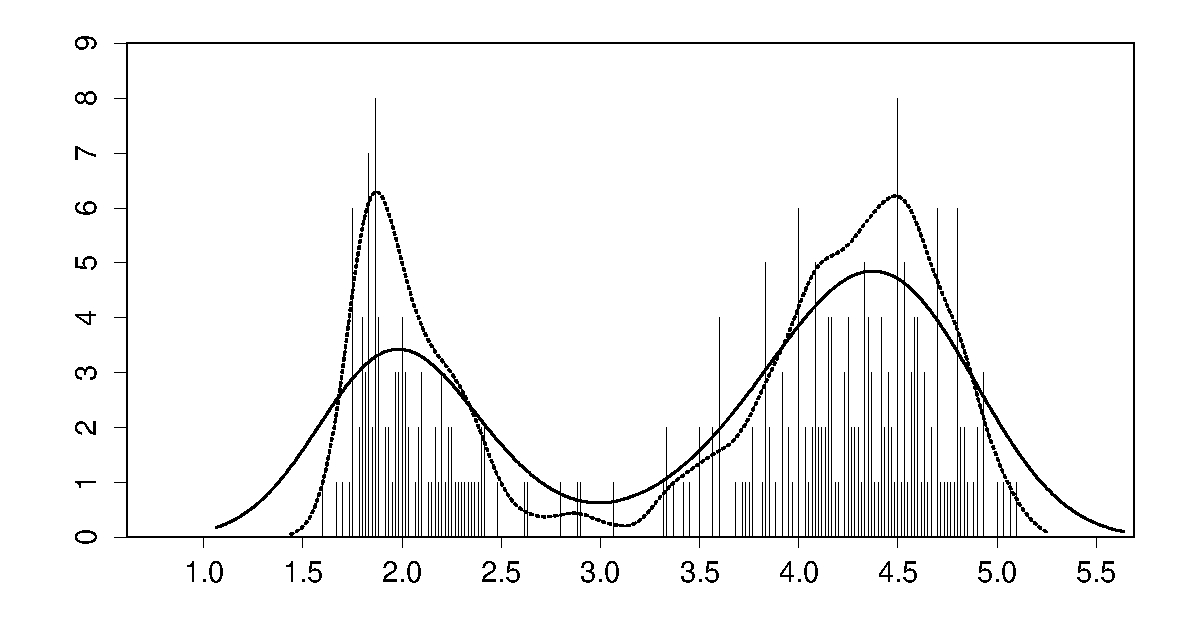
\includegraphics[width=.5\textwidth]{geys-2kern} %<< no file extension
  %%         --- .5\textwidth stands for 50% of text width
  \caption[Geyser data: binned histogram, Silverman's and another
  kernel]%<<-- Legend for the list of figures at the beginning of you thesis
  {Old Faithful Geyser eruption lengths, $n=272$; binned data and two
    (Gaussian) kernel density estimates ($\times 10$) with $h=h^*= .3348$
    and $h= .1$ (dotted).}% legend displayed below the graph.
  \label{fig:geys2}
\end{figure}

\section{To make a proof}
\begin{proof}
  $1 + 1 = 2$
\end{proof}

\section{To include \Rp code}
See information in Appendix~\ref{app:complement}.


\section{Other information}
Put a text between quotes: make sure to use nice quotes, such as ``quote''.

Cite a document in the bibliography (an example here): \cite{Reference}.
%%--> in file   myReferences.bib  (same directory)
Or mention that \citeauthor{HamF85} (a person) or \citeauthor{StaWW91} (two
persons) have already done quite a bit work.

Referencing a different part of your work: please refer to Appendix \ref{app:complement}.


%%% Local Variables: 
%%% mode: latex
%%% TeX-master: "MasterThesisSfS"
%%% End: 

%%\include{Chapter...}
\chapter{Summary}
\label{s:Summary}

Summarize the presented work. Why is it useful to the research field or institute?


\section{Future Work}
\label{ss:FutureWork}

Possible ways to extend the work.


%%% Local Variables: 
%%% mode: latex
%%% TeX-master: "MasterThesisSfS"
%%% End: 
 

%%%%%%%%%%%%%%%%%%%%%%%%%%%%%%%%%%%%%%%%%%%%%%%%%
%%% Bibliography                              %%%
%%%%%%%%%%%%%%%%%%%%%%%%%%%%%%%%%%%%%%%%%%%%%%%%%
\addtocontents{toc}{\vspace{.5\baselineskip}}
\cleardoublepage
\phantomsection
\addcontentsline{toc}{chapter}{\protect\numberline{}{Bibliography}}
\bibliography{myReferences}
%% All books from our library (SfS) are already in a BiBTeX file
%% (Assbib). You can use Assbib combined with your personal BiBTeX file:
%% \bibliography{Myreferences,Assbib}. Of course, this will only work on
%% the computers at SfS, unless you copy the Assbib file 
%%  --> /u/sfs/bib/Assbib.bib

%%%%%%%%%%%%%%%%%%%%%%%%%%%%%%%%%%%%%%%%%%%%%%%%% 
%%% Appendices (if needed)                    %%%
%%%%%%%%%%%%%%%%%%%%%%%%%%%%%%%%%%%%%%%%%%%%%%%%%
\addtocontents{toc}{\vspace{.5\baselineskip}}
\appendix
\chapter{Complementary information}
\label{app:complement}

Additional material. For example long mathematical derivations could be
given in the appendix. Or you could include part of your code that is
needed in printed form. You can add several Appendices to your thesis (as
you can include several chapters in the main part of your work).

\section{Including \Rp code with verbatim}
A simple way to include code or {\it R} output is to use
\texttt{verbatim}. It just prints the text however it is (including all
spaces, ``strange'' symbols,...) in a slightly different font.
\begin{verbatim}
## loading packages
library(RBGL)
library(Rgraphviz)
library(boot)

## global variables
X_MAX <- 150

   This allows me to put as many s  p a   c es   as I want.
I can also use \ and ` and & and all the rest that is usually only 
accepted in the math mode.

I can also make as 
                  many 
             line 
    breaks as 
I want... and
             where I want. 
\end{verbatim}

\section{Including \Rp code with the \emph{listings} package}
However, it is much nicer to use the \emph{listings} package to include \Rp
code in your report. It allows you to number the lines, color the comments
differently than the code, and so on.

\lstinputlisting{Pictures/picture.R}


\section{Using Sweave to include \Rp code (and more) in your report}
The easiest (and most elegant) way to include \Rp code and its output (and
have all your figures up to date with your report) is to use Sweave. You
can find an introduction Sweave in \texttt{/u/sfs/StatSoftDoc/Sweave/Sweave-tutorial.pdf}.

%%% Local Variables: 
%%% mode: latex
%%% TeX-master: "MasterThesisSfS"
%%% End: 

\chapter{Mathematical Identities}\label{app:math}

\section{Incremental Covariance Matrix Inverse}
% note the speedup expected
% In MATLAB backslash is optimized so speedup not observed.

The GP-update equations \eqref{gpUpdate_mu} and \eqref{gpUpdate_sigma}, require the inversion of the matrix $P_{t} \defeq K(x_{T}, x_{T}) + \sigma_{n}^{2}\mathbf{I}$. Since the CPG-UCB optimization \eqref{ucb} requires $\mu(x)$ and $\sigma(x)$ at each time step $t$, this matrix needs to be inverted at each step. The backlash operation to bypass this inversion requires $N^{3}/6$ complexity. For a single test point $x_{t}$, a workaround is to use incremental inverse for the growing matrix:

\begin{equation}
P_{t+1} = 
\left(
\begin{BMAT}(rc){c:c}{c:c}
P_{t} & k(x_{T}, x_{t}) \\
k(x_{T}, x_{t})^{\mathrm{T}} & k(x_{t}, x_{t})
\end{BMAT} 
\right)
\label{CovMat}
\end{equation}

where $k(x_{T}, x_{t}) \defeq (k(x_{1}, x_{t}), \ldots, k(x_{t-1}, x_{t	}))^{\mathrm{T}}$. 

The inverse of a general invertible $n \times n$ partitioned matrix 

\begin{equation*}
A = 
\left(
\begin{array}{cc}
P & Q \\
R & S \\
\end{array} 
\right)
\end{equation*}

is the $A^{-1}$ matrix:

\begin{equation*}
A^{-1} = 
\left(
\begin{array}{cc}
\tilde{P} & \tilde{Q} \\
\tilde{R} & \tilde{S} \\
\end{array} 
\right)
\end{equation*}

where the submatrices are given as \cite{GPbook}:

\begin{eqnarray}
\tilde{P} & = & P^{-1} + P^{-1}QMRP^{-1} \label{Phat}\\
\tilde{Q} & = & -P^{-1}QM \label{Qhat} \\
\tilde{R} & = & -MRP^{-1} \label{Rhat} \\
\tilde{S} & = & M \label{Shat}
\end{eqnarray}

and $M = (S - RP^{-1}Q)^{-1}$. Applying \eqref{Phat} - \eqref{Shat} on the inverse of the covariance matrix \eqref{CovMat} we get:

\begin{equation}
P_{t+1}^{-1} = 
\left(
\begin{BMAT}(rc){c:c}{c:c}
P_{t}^{-1} + \alpha P_{t}^{-1} q_{t} q_{t}^{\mathrm{T}} P_{t}^{-1}  & -\alpha P_{t}^{-1} q_{t} \\
-\alpha q_{t}^{\mathrm{T}} P_{t}^{-1} & \alpha
\end{BMAT} 
\right)
\label{CovMatInv}
\end{equation}

where 

\begin{eqnarray}
\alpha^{-1} & = & k(x_{t}, x_{t}) - q_{t}^{\mathrm{T}}P_{t}^{-1}q_{t} + \sigma_{n}^{2} \\
q_{t} & = & k(x_{t}, x_{T})
\end{eqnarray}

$\alpha$ is a scalar that is the outcome of the last point taken, $x_{t}$. \eqref{CovMatInv} can be reached easily by plugging the block matrices in \eqref{Phat} - \eqref{Shat} and noting that the covariance matrix $P_{t}$ is square symmetric.

A practical way to iteratively compute \eqref{CovMatInv} from $P_{t}^{-1}$ would be to compute first the vector of covariances $q_{t}$  and then $q_{t}^{\mathrm{T}}P_{t}^{-1}$, and apply it throughout the block matrices in \eqref{CovMatInv}. Figure \ref{fig:runtimes} shows the results for such an implementation in MATLAB running on Intel i7 1.6 GHz Quadcore laptop, where the runtimes for the matrix multiplication operation, $(K(x_{T}, x_{T}) + \sigma_{n}^{2}\mathbf{I})^{-1}\mathbf{k}_N(x^{*})$ is compared. The incremental matrix inversion is clearly faster, especially as the data sample size $N$ increases. Figure \ref{fig:deltaruntimes} shows the effect more clearly. Note that for the backslash method, the covariance matrix is not built from scratch at each iteration, but only the last row and column are added.

\begin{figure}
\center
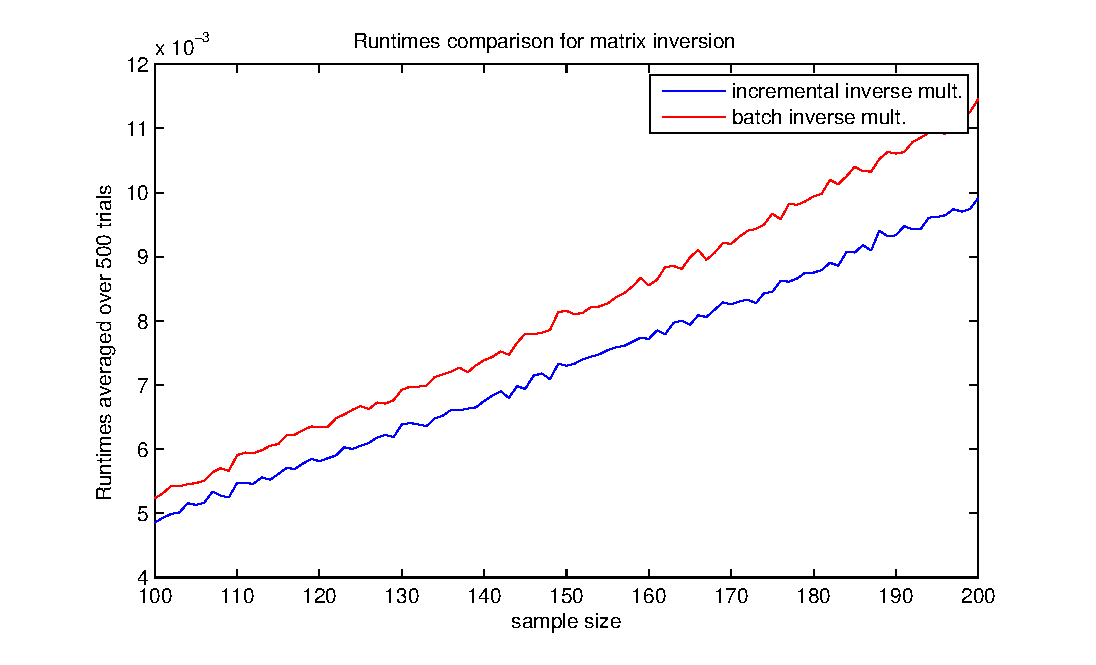
\includegraphics[scale=0.50]{runningtimes.eps}	
\caption{Runtime comparison}
\label{fig:runtimes}
\end{figure}

\begin{figure}
\center
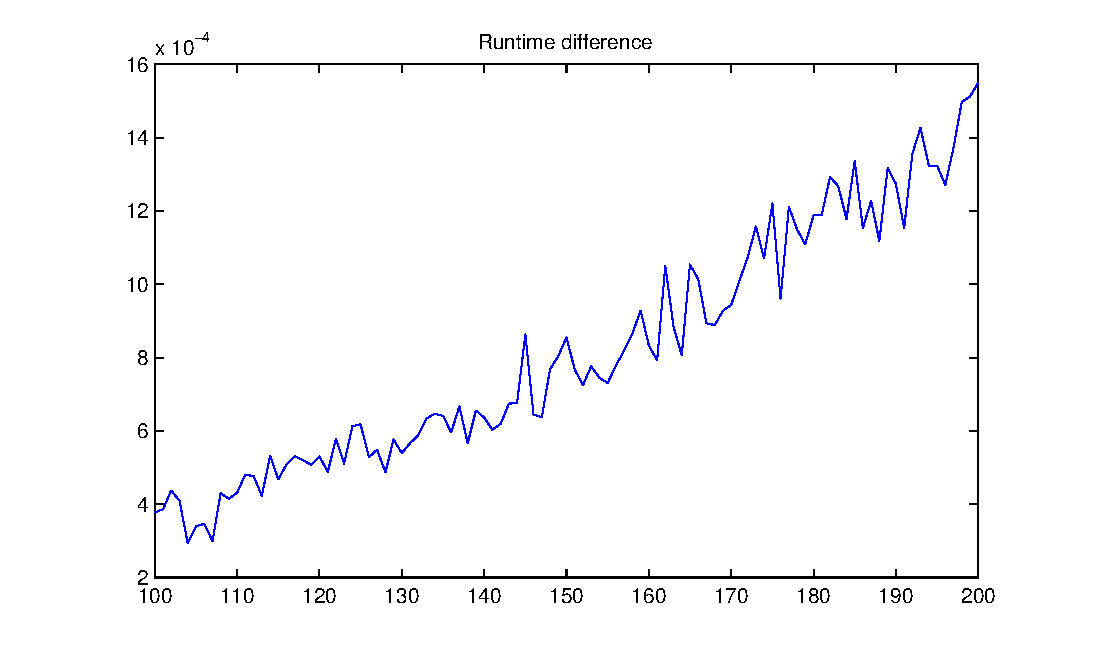
\includegraphics[scale=0.50]{delta_runningtimes.eps}	
\caption{Difference in runtimes}
\label{fig:deltaruntimes}
\end{figure}



%% Epilogue (optional)
\addtocontents{toc}{\vspace{.5\baselineskip}}
\cleardoublepage
\phantomsection
\addcontentsline{toc}{chapter}{\protect\numberline{}{Epilogue}}
\markboth{Epilogue}{Epilogue}
\chapter*{Epilogue}
\label{s:Epilogue}

A few final words.



%%% Local Variables: 
%%% mode: latex
%%% TeX-master: "MasterThesisSfS"
%%% End: 


\end{document}
